\documentclass[UTF8]{ctexart}
\usepackage{amsmath}
\usepackage{amssymb}
\usepackage{booktabs}
\usepackage{background}
\usepackage{caption,subcaption}
\usepackage{CJKfntef}
\usepackage{cprotect}
\usepackage{enumitem}
\usepackage{fancyhdr}
\usepackage{float}
\usepackage{fontspec}
%\usepackage{fourier}
\usepackage{geometry}
\usepackage{listings}
\usepackage{tcolorbox}
\tcbuselibrary{breakable}
\usepackage{tikz}
\usetikzlibrary{arrows.meta}
\usepackage[table]{xcolor}

\geometry{a5paper, top=0.1cm, left=1cm, right=1cm, bottom=1cm, footskip=0.1cm}
\setCJKmainfont[BoldFont={汉仪文黑-85W},ItalicFont={方正苏新诗柳楷简体}]{汉仪文黑-55W}
\setfontfamily\Issue{Century Schoolbook}
\setfontfamily\Genshin{Genshin Teyvat Lingua Franca}
\newCJKfontfamily\TitleFont{思源宋体 CN Heavy}
\newfontfamily\timesnewroman{Times New Roman}
%\reversemarginpar

\pagestyle{fancy}
\fancyhf{}
\cfoot{\sffamily\footnotesize{-\ \thepage\ -}}
%\CTEXsetup[format = {\centering\bfseries\large}, beforeskip = 3pt, afterskip = 3pt]{section}

\colorlet{darkcyan}{cyan!50!black}
\newcommand\Black[1]{\textcolor[gray]{0.3}{#1}}
\newcommand\Brown[1]{\textcolor[HTML]{998A4E}{#1}}
\newcommand\Emph[1]{\colorbox{green!10}{\textcolor{green!30!black}{#1}}}
\newcommand\Notes[1]{\textcolor{yellow!50!black}{\small #1}}
\newcommand\Example[1]{\textcolor{cyan!70!black}{\small #1}}
\newcommand\keyword[1]{\textcolor{violet}{\textbf{\texttt{#1}}}}

\newcommand\littleword[1]{\textcolor{gray}{\footnotesize #1}}

\lstset{
    basicstyle=\small\ttfamily, %注意行末有逗号!
    keywordstyle=\bfseries\color{blue!70!black},
    commentstyle=\color{cyan!90!black},
    stringstyle=\color{green!40!black},
    columns=flexible,
    numbers=left,
    numberstyle=\footnotesize,
    escapechar=`,
    frame=shadowbox,
    %rulesepcolor=\color{red!20!blue!20!green!20}
    backgroundcolor=\color{cyan!5!white},
    language = C++,
    tabsize = 4,
    breaklines = true,
    showstringspaces = false,
}

\newcommand\IssueNumber{34}
\newcommand\Date{2024-9-18}
%\newcommand\Contributer{@金光日}
\newcommand\Subject{计算机组成原理}


\begin{document}
\backgroundsetup{contents=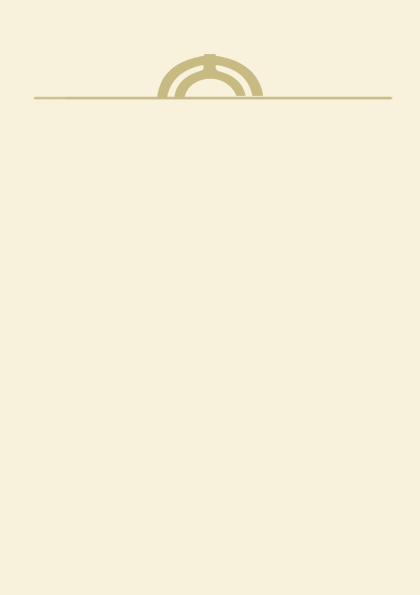
\includegraphics{上半示例.png}, center, scale=1, angle=0, opacity=1}
\BgThispage
\begin{center}
%{\scriptsize\Issue \textcolor[HTML]{C8BA83}{\Genshin WEEKLY TIPS}}
\phantom{...}

{\Large\textcolor{brown!40!white}{\makebox[10cm][s]{\Genshin WEEKLY KNOWLEDGE TIPS}}}

\vspace{-2em}

{\Huge\bfseries\TitleFont \Black{知\ 识\ 小\ 料}}


\vspace{-0.1cm}
{\footnotesize \Brown{「电计 2203 班」周常规知识整理共享}}
\end{center}

\vspace{-0.5cm}


\begin{figure}[H]
\hspace{1cm}
\begin{minipage}[t]{0.3\textwidth}
\centering
    \Brown{\Genshin ISSUE}

    \vspace{-0.6cm}
    \Huge \Issue\slshape\bfseries\Black{\IssueNumber}
\end{minipage}
\hfill
\begin{minipage}[t]{0.35\textwidth}
\centering
    \Brown{日期:\Date} \\
%\vspace{-0.1cm}
%    \Brown{贡献者:\Contributer} \\
\vspace{-0.1cm}
    \Brown{学科:\Subject} \\
\end{minipage}
\hspace{0.8cm}
\end{figure}

{\color{cyan!50!black}
从十进制的角度看二进制浮点数补码加法。假设 $x=0.1100\times 2^{011}$,$y=-0.0110\times 2^{110}$,求 $x+y$ 。阶码三位,尾数六位。
}

\begin{table}[htb]
  \centering
  \begin{tabular}{crccccccc@{\qquad}c}
  & & \littleword{$\frac12$} &  \littleword{$\frac14$} &  \littleword{$\frac18$} &  \littleword{$\frac{1}{16}$} & \littleword{$\frac{1}{32}$} & \littleword{$\frac{1}{64}$} \\
  $x=$ & $0.$ & 1 & 1 & 0 & 0 & 0 & 0 & $\times 2^{011}$ & \textcolor{violet}{$\frac34\times 2^3$}\\
  $y=$ & $-0.$ & 0 & 1 & 1 & 0 & 0 & 0 & $\times 2^{110}$ & \textcolor{violet}{$-\frac{3}{8}\times 2^6$}\\
  \end{tabular} 
  
  
  \begin{tabular}{cc@{\ ,\ }c@{\quad ;\quad }c@{\ ,\ }c}
    & \multicolumn{2}{c}{\littleword{阶码}} & \multicolumn{2}{c}{\littleword{尾数}} \\
    $[x]_{\text{补}} = $ & 00 & 011 & 00 & 110000 \\
    $[y]_{\text{补}} = $ & 00 & 110 & 11 & 101000 \\
  \end{tabular}
\end{table}

(注:$y$ 的原码 $11,011000$ $\to$ 反码 $11,100111$ $\to$ 补码 $11,101000$。)


\paragraph{第一步:对阶} 
用 $j$ 表示阶码,$j_x = (011)_2 = 3$,$j_y = (110)_2 = 6$,很明显 $j_x-j_y=-3$。当然也可以用补码竖式计算:

$[j_x]_{\text{补}} = 00,011$,$[j_y]_{\text{补}} = 00,110$,$[-j_y]_{\text{补}} = 11,010$——
\begin{table}[htb]
  \centering
  \begin{tabular}{lr@{\quad}c@{\ ,\ }c}
      & $[j_x]_{\text{补}}$ & 00 & 011 \\
  $+$ & $[-j_y]_{\text{补}}$ &11 & 010 \\
  \hline
      & & 11 & 101 \\
  \end{tabular}
\end{table}

(补码 $11,101$ $\to$ 反码 $11,100$ $\to$ 原码 $11,011$ $\to$ 真值 $-3$。)

因此应该把 $x$ 的阶码提高 3,使 $x$ 拥有和 $y$ 相同的阶码。可以看到,「改变阶码」这一操作伴随着尾数整体右移 3 位,但不改变原始数值。

\begin{table}[htb]
  \centering
  \begin{tabular}{cccccccccc|ccc}
  & & & & \littleword{$\frac12$} & \littleword{$\frac14$} & \littleword{$\frac18$} & \littleword{$\frac1{16}$} & \littleword{$\frac1{32}$} & \littleword{$\frac1{64}$} & & &\\
  $[x]_{\text{补}}=$ & 00 ,& 011 ;& 00 ,& 1&1&0&0&0&0 & \textcolor{violet}{$\frac34$} & \textcolor{violet}{$\times$} & \textcolor{violet}{$2^3$} \\
  & & $(+3)$ & & \multicolumn{6}{c}{$(>>3)$} & \textcolor{violet}{$(\div 2^3)$} & & \textcolor{violet}{$(\times 2^3)$}\\
  $[x]_{\text{补}}=$ & 00 ,& 100 ;& 00 ,& 0&0&0&1&1&0 & \textcolor{violet}{$\frac{3}{32}$} & \textcolor{violet}{$\times$} & \textcolor{violet}{$2^6$} \\
  \end{tabular}
\end{table}


\paragraph{第二步:尾数求和} 用 $S$ 表示尾数,$[S_x]_{\text{补}} = 00,000110$,$[S_y]_{\text{补}} = 11,101000$ ,做加和——
\begin{table}[htb]
  \centering
  \begin{tabular}{lr@{\quad}c@{\ ,\ }c@{\qquad}c}
      & $[S_x]_{\text{补}}$ & 00 & 000110 & \textcolor{violet}{$\frac3{32}$}\\
  $+$ & $[S_y]_{\text{补}}$ & 11 & 101000 & \textcolor{violet}{$-\frac{3}{8}$}\\
  \hline
      & & 11 & 101110 & \textcolor{violet}{$-\frac{9}{32}$}\\
  \end{tabular}
\end{table}

(补码 $11,101110$ $\to$ 反码 $11,101101$ $\to$ 原码 $11,010010$ $\to$ 真值 $-\frac{9}{32}$。)

\backgroundsetup{contents=
\includegraphics{下半示例.png}, center, scale=1, angle=0, opacity=1}
\BgThispage
因此 $x+y$ 补码的尾数就是 $11,101110$。

\begin{table}[htb]
  \centering
  \begin{tabular}{cc@{\ ,\ }c@{\quad ;\quad }c@{\ ,\ }c@{\qquad}c}
    & \multicolumn{2}{c}{\littleword{阶码}} & \multicolumn{2}{c}{\littleword{尾数}} & \\
    $[x+y]_{\text{补}} = $ & 00 & 110 & 11 & 101110 & \textcolor{violet}{$-\frac{9}{32}\times 2^6$} \\
  \end{tabular}
\end{table}

\paragraph{第三步:检查规格化} 补码规格化的要求是,尾数的第一位和符号位相反,也就是 $11,0\text{xxxxx}$。但是,我们得到的尾数是 $11,101110$,不符合规格化要求,因此需要:
\begin{itemize}[itemsep=0pt,parsep=0pt]
  \item 尾数整体左移一位\textcolor{violet}{$(\times 2^1)$},左移\textcolor{green!70!black}{补进零};
  \item 阶码减一\textcolor{violet}{$(\times 2^{-1})$}。如此即可保证\textcolor{violet}{原始数值不变}。
\end{itemize}

\begin{table}[htb]
  \centering
  \begin{tabular}{cccccccccc|ccc}
  & & & & \littleword{$\frac12$} & \littleword{$\frac14$} & \littleword{$\frac18$} & \littleword{$\frac1{16}$} & \littleword{$\frac1{32}$} & \littleword{$\frac1{64}$} & & &\\
  $[x+y]_{\text{补}}=$ & 00 ,& 110 ;& 11 ,& 1&0&1&1&1&0 & \textcolor{violet}{$-\frac{9}{32}$} & \textcolor{violet}{$\times$} & \textcolor{violet}{$2^6$} \\
  & & $(-1)$ & & \multicolumn{6}{c}{$(<<1)$} & \textcolor{violet}{$(\times 2^1)$} & & \textcolor{violet}{$(\times 2^{-1})$}\\
  $[x+y]_{\text{补}}=$ & 00 ,& 101 ;& 11 ,& 0&1&1&1&0&\textcolor{green!70!black}{0} & \textcolor{violet}{$-\frac{9}{16}$} & \textcolor{violet}{$\times$} & \textcolor{violet}{$2^5$} \\
  \end{tabular}
\end{table}

(补码 $11,011100$ $\to$ 反码 $11,011011$ $\to$ 原码 $11,100100$。)

该过程是左移,不存在「零舍一入」的问题;也不会产生溢出。

因此 $x+y$ 的原码即为 $00,101; 11,100100$,真值为 $-\frac{9}{16}\times 2^5$ 即二进制 $-0.1001\times 2^{101}$。

\vspace{1em}

{\color{cyan!80!black} 【结论】$-0.1001\times 2^{101}$。

【点评】本题用于复习浮点数的加减法问题,综合使用了小数二进制的转换、原反补三码的转换、求相反数补码、浮点数的规格化等知识。本文档旨在给出每一步的十进制表示,便于同学们理解这种方法的「原始数值」的不变性。
}

\end{document}